\documentclass[tikz,border=2pt]{standalone}

\usepackage{amsmath}
\usepackage{xcolor}
\usepackage{newtxtext}
\usepackage{tikz}
\usetikzlibrary{arrows.meta,positioning,fit,backgrounds,calc,decorations.pathreplacing,patterns,shapes.geometric}
\usepackage{pgfplots}
\pgfplotsset{compat=1.18}
\usepgfplotslibrary{groupplots,fillbetween}

\definecolor{bestcolor}{HTML}{E8F5E9}
\definecolor{gaincolor}{HTML}{1B5E20}
\definecolor{cStandard}{HTML}{BF616A}
\definecolor{cAOI}{HTML}{5E81AC}
\definecolor{cDelta}{HTML}{A3BE8C}
\definecolor{cVisual}{HTML}{D08770}
\definecolor{cASR}{HTML}{B48EAD}
\definecolor{cNarr}{HTML}{88C0D0}
\definecolor{cAccent}{HTML}{EBCB8B}
\definecolor{cGray}{HTML}{4C566A}
\definecolor{cLightGray}{HTML}{D8DEE9}

\begin{document}
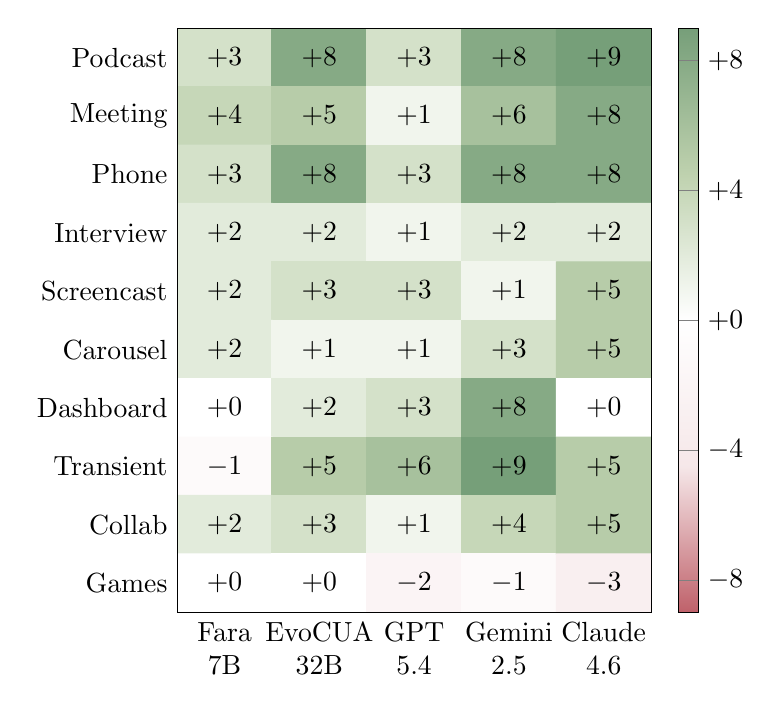
\begin{tikzpicture}
\begin{axis}[
    width=7.6cm,
    height=9.0cm,
    enlargelimits=false,
    axis on top,
    colormap={div}{
        color=(cStandard)
        color=(cStandard!15)
        color=(white)
        color=(cDelta!70)
        color=(gaincolor!60)
    },
    point meta min=-9,
    point meta max=9,
    xtick={0,1,2,3,4},
    xticklabels={
        {Fara\\7B},
        {EvoCUA\\32B},
        {GPT\\5.4},
        {Gemini\\2.5},
        {Claude\\4.6}
    },
    xticklabel style={
        font=\normalsize,
        align=center
    },
    ytick={0,1,2,3,4,5,6,7,8,9},
    yticklabels={
        Podcast,
        Meeting,
        Phone,
        Interview,
        Screencast,
        Carousel,
        Dashboard,
        Transient,
        Collab,
        Games
    },
    yticklabel style={
        font=\normalsize,
        anchor=east
    },
    xtick style={draw=none},
    ytick style={draw=none},
    y dir=reverse,
    nodes near coords={
        \pgfmathprintnumber[print sign]\pgfplotspointmeta
    },
    nodes near coords style={
        font=\normalsize\bfseries,
        anchor=center,
        text=black
    },
    colorbar,
    colorbar style={
        width=7pt,
        font=\normalsize,
        ytick={-8,-4,0,4,8},
        yticklabel={
            \pgfmathprintnumber[print sign]\tick
        }
    },
]

\addplot[
    matrix plot*,
    mesh/cols=5,
    point meta=explicit
] coordinates {
    % Podcast
    (0,0)[3]  (1,0)[8]  (2,0)[3]  (3,0)[8]  (4,0)[9]

    % Meeting
    (0,1)[4]  (1,1)[5]  (2,1)[1]  (3,1)[6]  (4,1)[8]

    % Phone
    (0,2)[3]  (1,2)[8]  (2,2)[3]  (3,2)[8]  (4,2)[8]

    % Interview
    (0,3)[2]  (1,3)[2]  (2,3)[1]  (3,3)[2]  (4,3)[2]

    % Screencast
    (0,4)[2]  (1,4)[3]  (2,4)[3]  (3,4)[1]  (4,4)[5]

    % Carousel
    (0,5)[2]  (1,5)[1]  (2,5)[1]  (3,5)[3]  (4,5)[5]

    % Dashboard
    (0,6)[0]  (1,6)[2]  (2,6)[3]  (3,6)[8]  (4,6)[0]

    % Transient
    (0,7)[-1] (1,7)[5]  (2,7)[6]  (3,7)[9]  (4,7)[5]

    % Collab
    (0,8)[2]  (1,8)[3]  (2,8)[1]  (3,8)[4]  (4,8)[5]

    % Games
    (0,9)[0]  (1,9)[0]  (2,9)[-2] (3,9)[-1] (4,9)[-3]
};

\end{axis}
\end{tikzpicture}
\end{document}
